\chapter{Result}
\section{Experimentations}
The experimentation based on a machine equipped with Intel(R) Core(TM) i7-4790 CPU 3.6GHz, 16 GB of RAM. The testing data is two set of biological images: \textit{Right mandible and left mandible}. For each dataset, it includes 293 images(3264 x 2448). However, the data was filtered by suppressing the bad images in both dataset. The bad images includes the empty images and broken images (image contains the broken object). They are showed as below:
\begin{multicols}{3}
\begin{itemize}
\item Md 004.JPG
\item Md 146.JPG
\item Md 238.JPG
\item Mg 003.JPG
\item Mg 007.JPG
\item Mg 040.JPG
\item Mg 066.JPG
\item Mg 159.JPG
\item Mg 248.JPG
\item Mg 292.JPG
\end{itemize} 
\end{multicols}
\subsection{Parameters}
In the program, we have used the parameters for the methods:
\begin{itemize}
\item The best segmentation obtained from choosing a good threshold value. In program, Canny algorithm used to segment the image. So, the ratio between \textit{lower threshold : upper threshold} is important to get a good result. And the ratio used: \textit{1 : 3} (in class \texttt{Image}, method \texttt{getEdges}), this ratio has been chosen experimentally. The lower value is 1 * \textit{threshold} value and the upper value is 3 * \textit{threshold} value. The \textit{threshold} value has been identified by analysing the histogram of image. 
\item The angle and distance accuracy used in constructing the PGH matrix and calculate the measure distance between PGHs. The angle accuracy can be 90 (0.5 * 180), 180, 360 (2 * 180), 720(4 * 180), 1080(6 * 180), 2160(12 * 180) degree. The distance accuracy can be 250, 500 or 1000 columns. The \textbf{default value} in program is \textbf{180} degree for angle accuracy, and \textbf{250} for the distance accuracy. 
\item During apply the Probabilistic Hough Transform, to save processing time during training, we just consider the pair of closet lines. And the parameters used to indicate the closet line are (used in method \texttt{closetLine}, class \texttt{PHoughTransform} ):
	\begin{itemize}
		\item Length of each line greater than \textbf{60} pixels
		\item Angle between two lines greater than \textbf{15} degree
		\item Perpendicular distance from one of two endpoints of a line to other line less than \textbf{5} pixel.
	\end{itemize}
The conditions to predicate two pairs of lines are similar (used in method \texttt{similarPairLines}, class \texttt{PHoughTransform}):
	\begin{itemize}
		\item Subtraction between angle of two pair of lines is less than \textbf{1}
		\item Subtraction between ratio couple of scene lines and reference lines is less than \textbf{1}
		\item Subtraction between distance of two pair of lines is less than \textbf{2}
	\end{itemize}
\item The size of bounding box around reference landmarks used for estimating landmarks by cross-correlation method or compute the estimated centroid is \textit{400} pixels (used in method \texttt{crossCorrelation and crossCorrelationDistance}, class \texttt{ImageViewer})
\item The size of bounding box around reference landmarks and estimated landmarks used to refine the estimated landmarks or compute the estimated centroid are \textit{400} pixels and \textbf{1400} pixels, respective.(used in method \texttt{getLandmarks and tplMatchingDistance}, class \texttt{ImageViewer})
To increase the flexible of program, all parameters was placed in the resources files (\textbf{data/resources} folder). For each group parameters, it was putted in a file, it can be easy to manage.
\end{itemize}
\section{Results}
The automated landmark identification is examined on two data sets. And the landmarks are extracted: 18 landmarks for each \textit{right mandible} image, 16 landmarks for each \textit{left mandible} image.\\[0.3cm]
\begin{figure}[h!]
\centering
\subfloat[The scene image]{\label{fig:pht_1}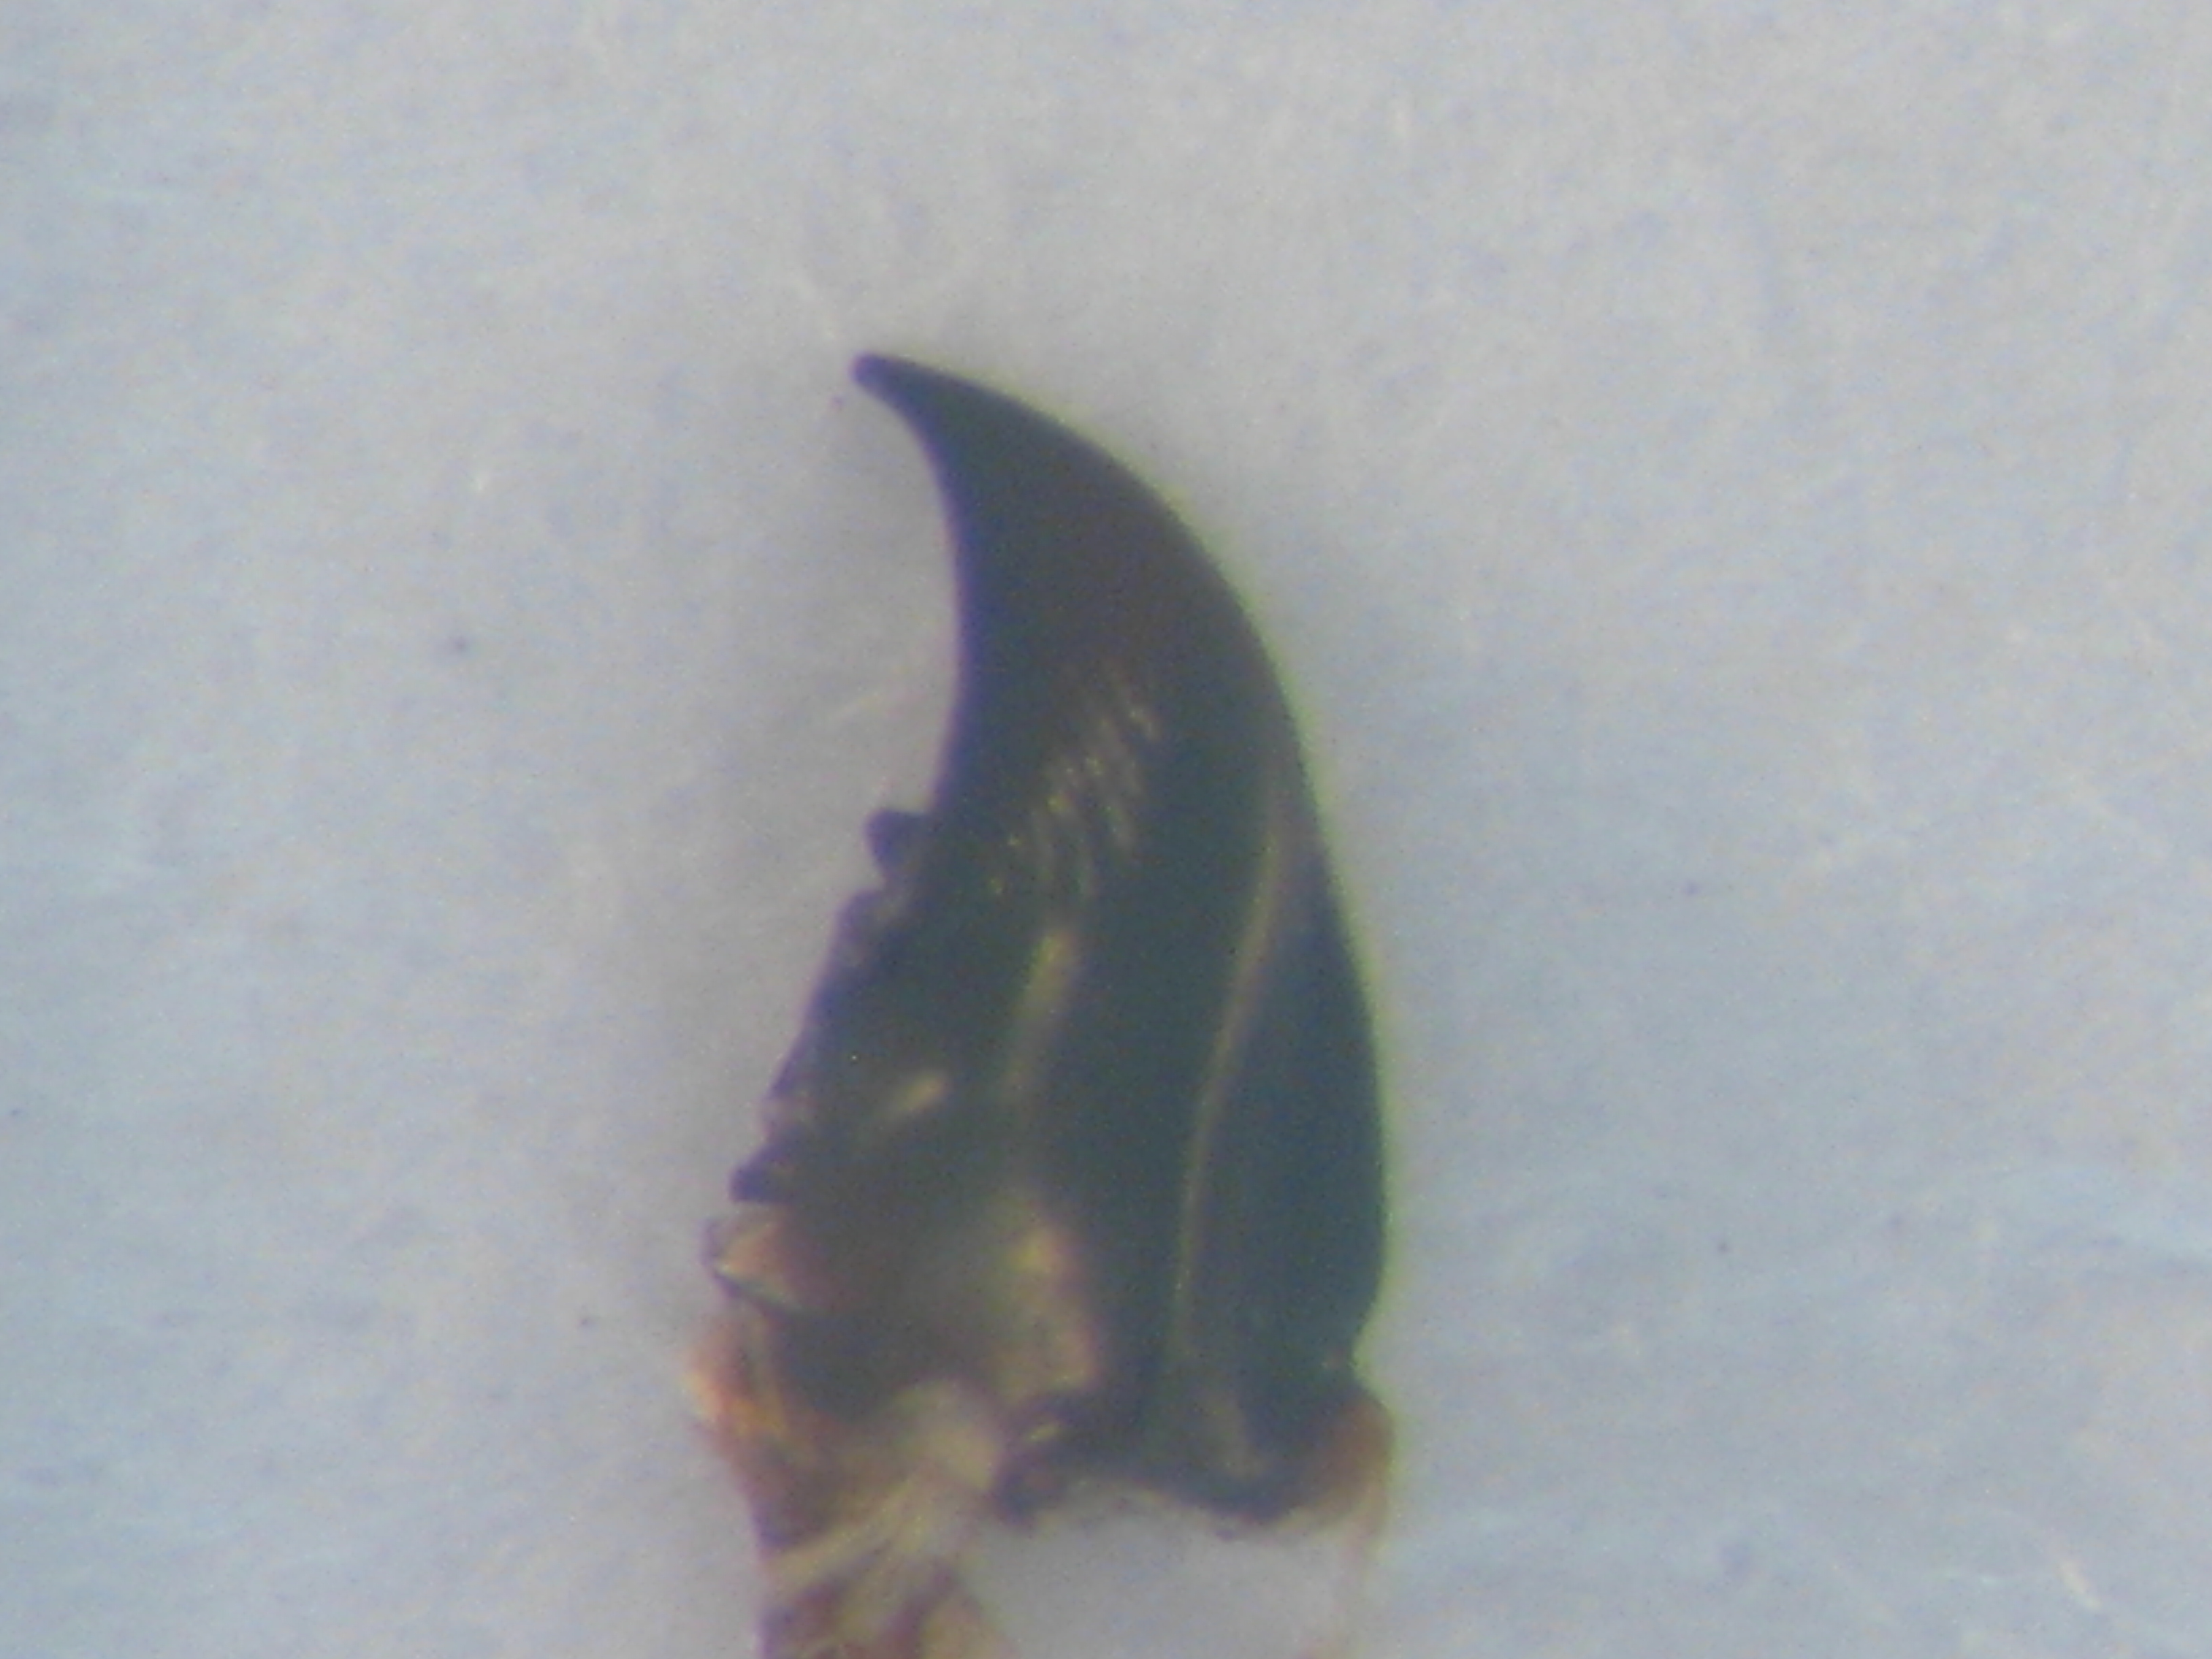
\includegraphics[width=0.45\textwidth]{./images/md32}}~~
\subfloat[The scene image with estimated landmarks ]{\label{fig:pht_2}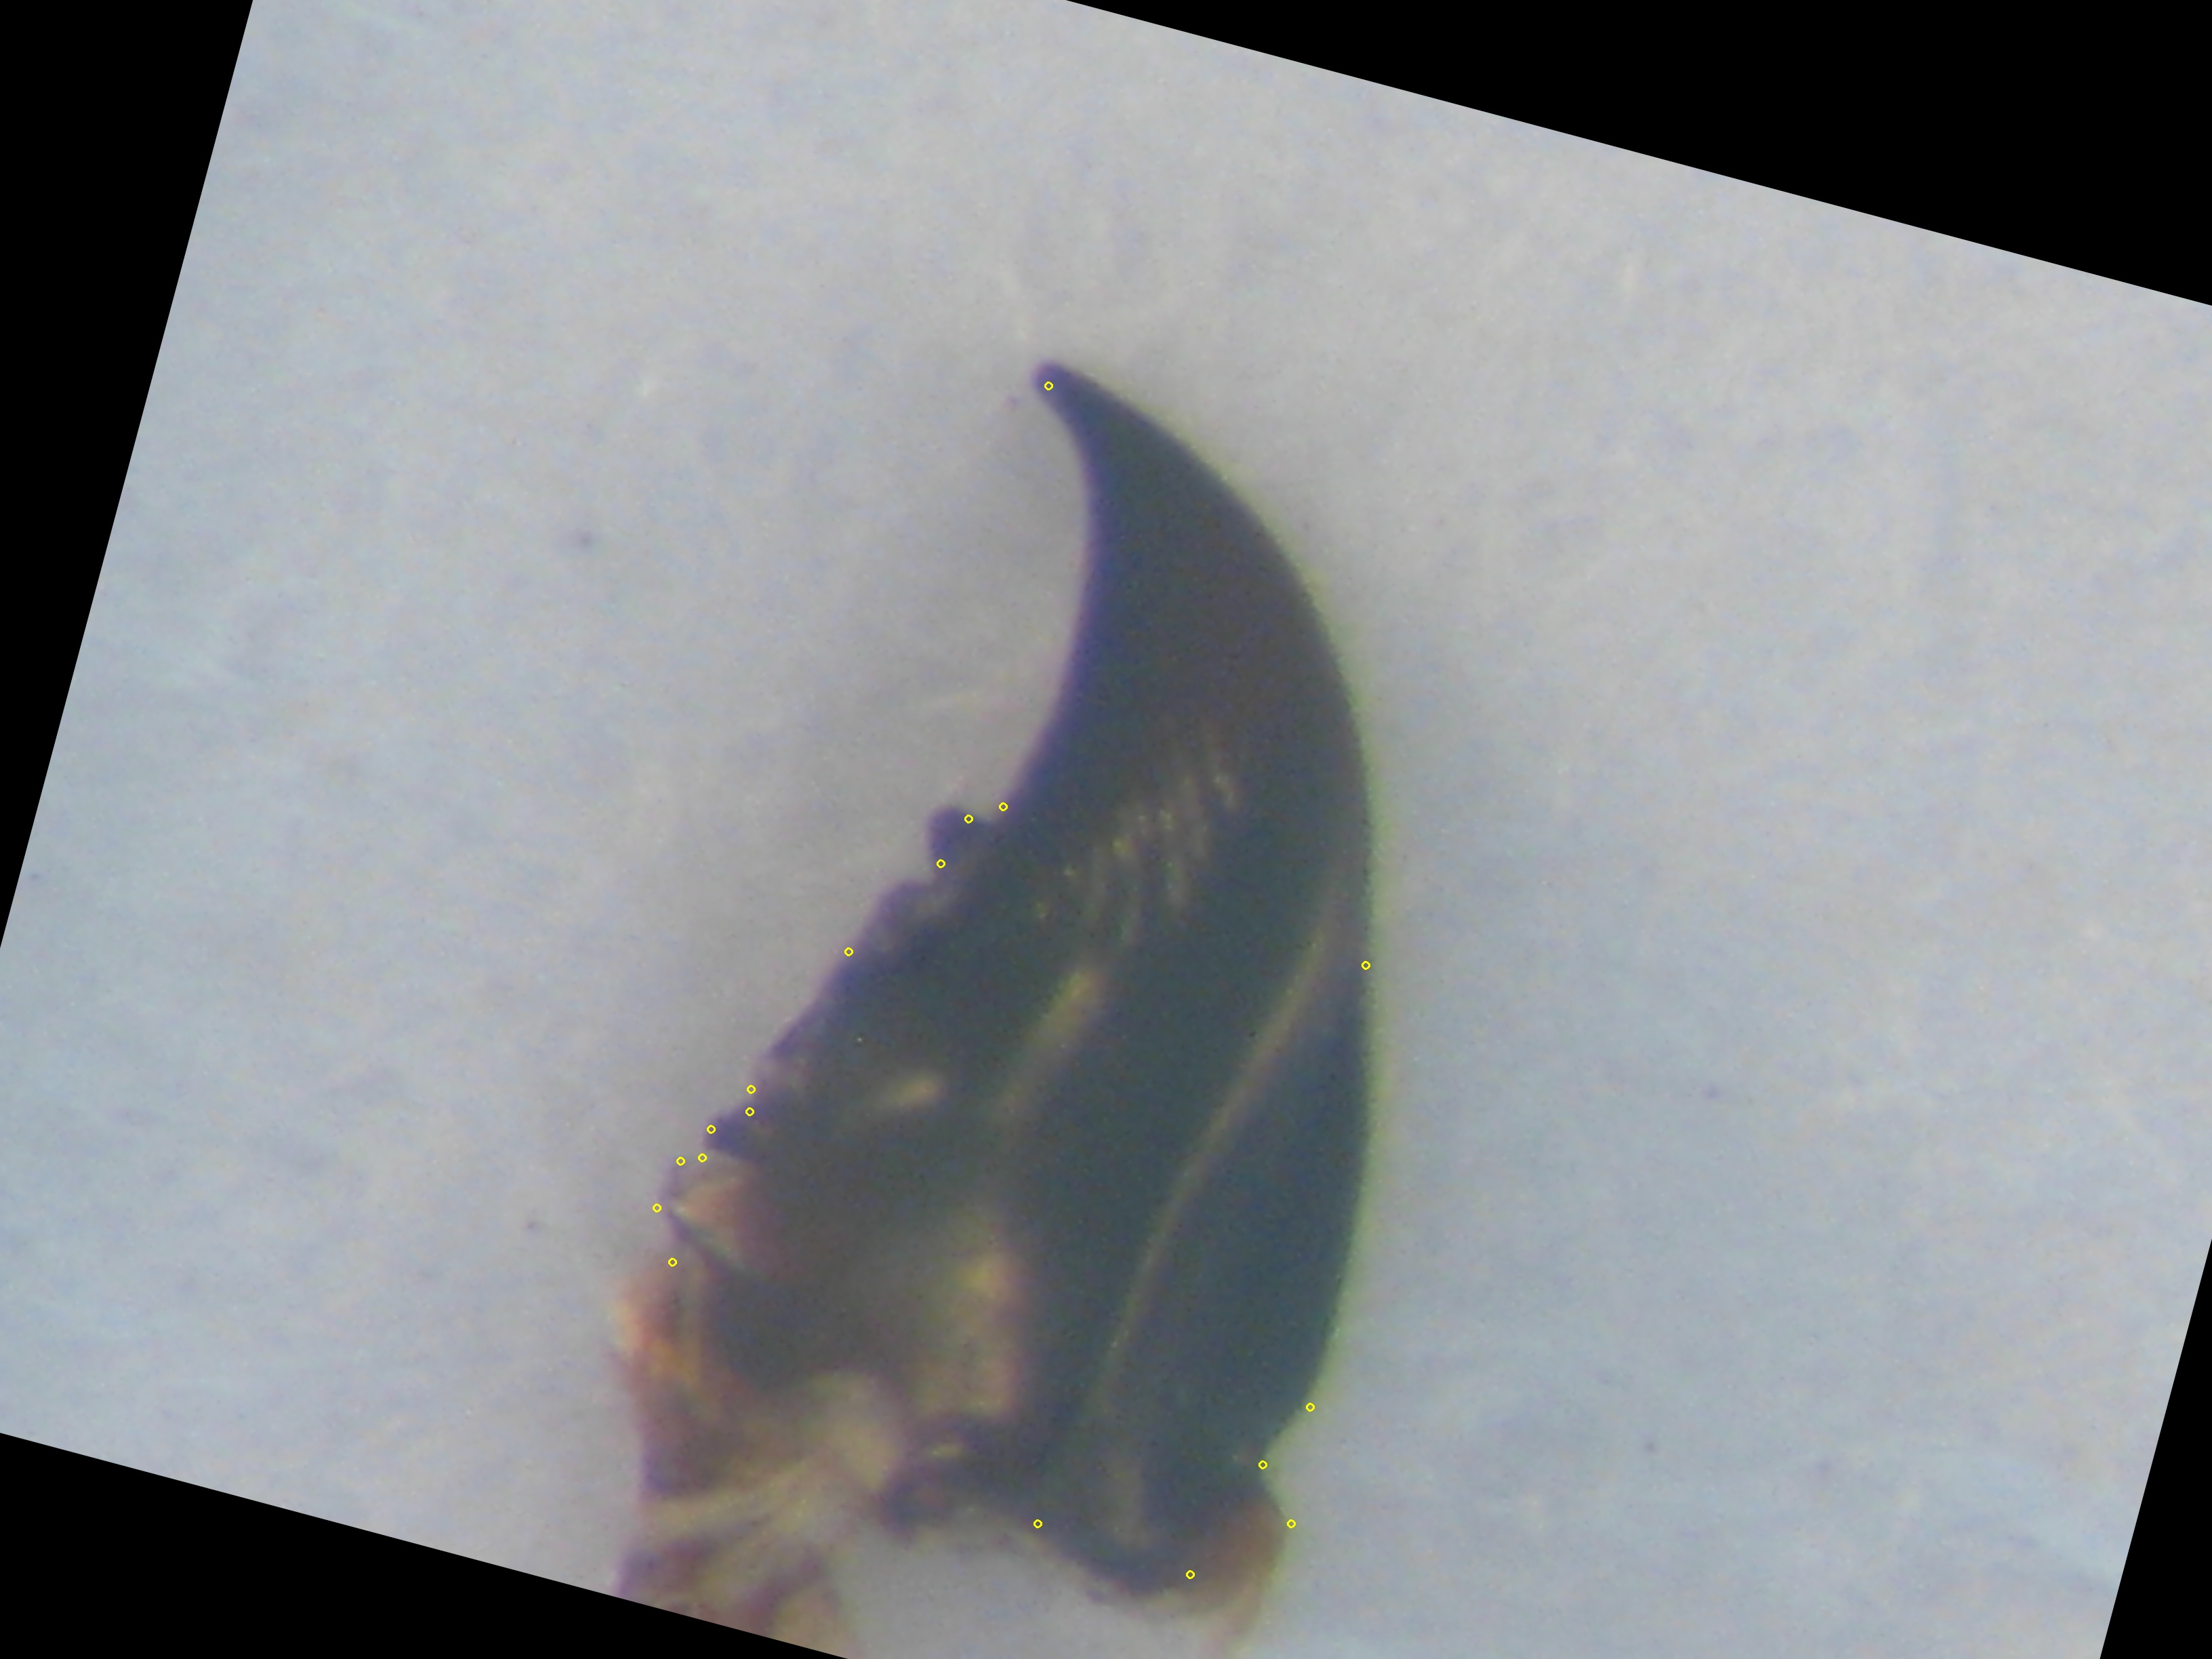
\includegraphics[width=0.45\textwidth]{./images/est32}}
\caption{Automatic identification the landmarks}
\label{fig:figure_31}
\end{figure}
The accuracy of system can be determined by comparing the differences(in pixels) between the landmarks located by this method and the manual landmarks. Besides, this method includes several steps, the result of each step will effect on next steps. So, to evaluate the accuracy of this method, we can evaluate the result of each step.\\